\documentclass[a4paper,11pt]{article}

\usepackage[utf8]{inputenc}
\usepackage[british]{babel}
\usepackage{csquotes}
\usepackage[style=apa]{biblatex}
\usepackage{graphicx}
\usepackage{float}
\usepackage{algorithm}
\usepackage[noend]{algpseudocode}

\bibliography{project-specification}

\graphicspath{{images/}}

\makeatletter
\def\BState{\State\hskip-\ALG@thistlm}
\makeatother

\begin{document}

\title{FIT3036 --- Project Specification}
\author{Dylan Pinn --- 24160547}
\maketitle
\pagebreak

\tableofcontents
\pagebreak

\section{Introduction}

This project specification outlines the plan to design, implement, test and
deliver the FIT3036 Computer Science project. We have been tasked to calculate
the total surface area of all of the roads within any given 1 square kilometre
space. We follow the software development life cycle for planning, creating
testing and deployment of the system. This will help ensure that that project
meets all of the requirements, is tested and is delivered on time.

\section{Project Requirements}

The functional and non-functional requirements of the project have been outlined
in the following sections.

\subsection{Functional Requirements}

The functional requirements are:

\begin{itemize}
  \item System shall allow a user to select a 1 square km area on Google Maps.
  \item System shall allow a user to request the total area of the roads within
    the nominated square area.
\end{itemize}

\subsection{Non-functional Requirements}

The non-functional requirements are:

\begin{itemize}
  \item System shall be easily accessible via the Internet.
  \item System shall be testable.
  \item System shall be affordable to host.
  \item System shall be easy to deploy.
  \item System shall be easy to maintain.
  \item System shall be well documented.
\end{itemize}

\section{Project Plan}

The project plan includes an overview of the project, risk analysis, resource
requirements and the project schedule.

\subsection{Overview}

\paragraph{Project Objectives:}

Our company secured a contract for a local council in Victoria to re-surface
roads in a designated kilometre area. The objectives are to design, implement,
test and deliver a system that will perform these calculations and display the
result to the user.

\paragraph{Requirements:}

We are to use Google Maps and related products and any satellite/aerial views.
The project involves writing the related code, with an elegant GUI to support
calculations. \autocite[2]{intro:1}

\paragraph{Constraints:}

We have the following constraints on the project:

\begin{itemize}
  \item Only have access to publicly available data.
  \item Limited to available information online.
  \item No / Limited access to council records.
  \item Project must be finalised by the end of week 12.
\end{itemize}

\subsection{Risk Analysis}

We have performed a risk analysis of the project and these and are outlined in
figure~\ref{fig:risk-register}. This includes the probability, potential
responses and impact to the project.

\begin{figure}[H]
  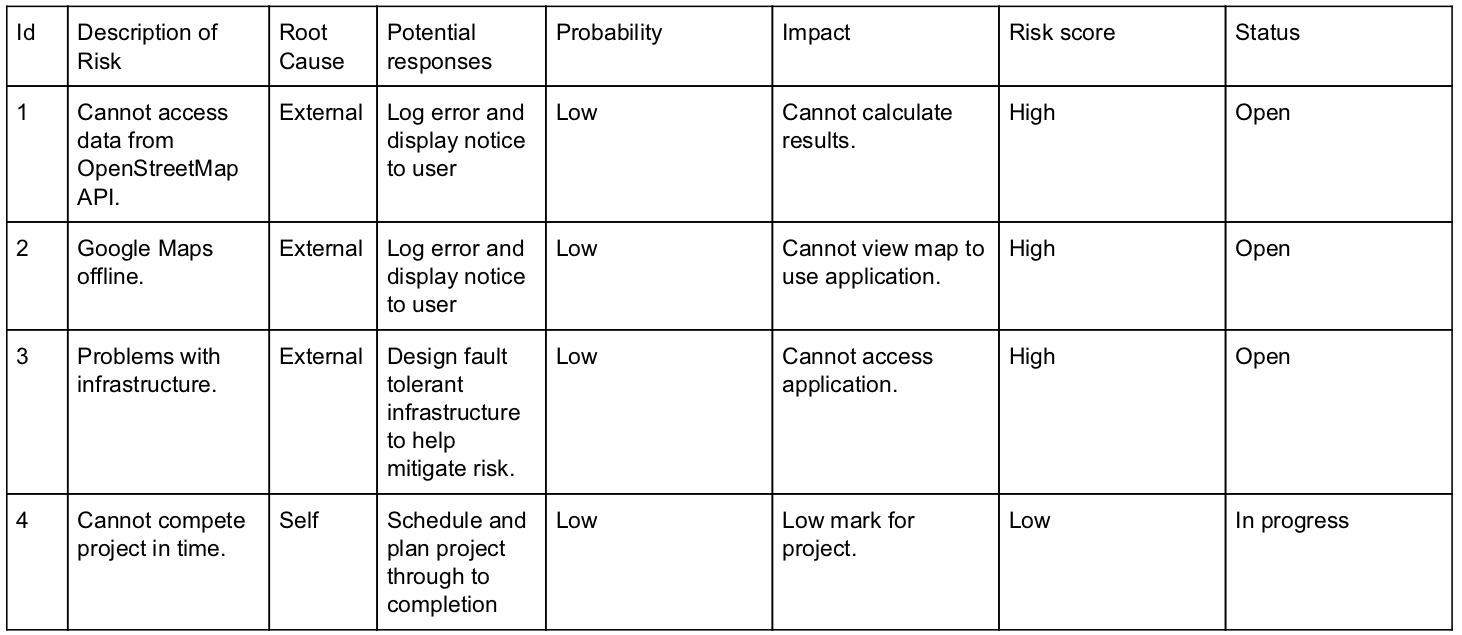
\includegraphics[width=\textwidth]{risk-register}
  \caption{Risk Register}\label{fig:risk-register}
\end{figure}

\subsection{Resource Requirements}

\paragraph{Hardware:}

We have decided to use as much Software as a Service (SaaS), Platform as a
Service (PaaS) and Infrastructure as a Service (IaaS) solutions to keep costs
down.

Amazon Web Services (AWS) has been chosen to use due to its comprehensive free
tier and prior experience with the platform. The following AWS services are
going to be utilised:

\begin{itemize}
  \item AWS Lambda --- Functions as service; allows running back-end code
    without maintaining server infrastructure \autocite{aws:2}.
  \item AWS API Gateway --- Allows creating public API endpoints for Lambda
    functions \autocite{aws:3}.
  \item AWS S3 --- Cheap scalable storage to store front-end code
    \autocite{aws:4}.
  \item AWS Cloudfront --- CDN for front-end code. Speeds up delivery by caching
    content \autocite{aws:5}.
  \item AWS Cloudformation --- Service to provision services on AWS
    \autocite{aws:6}
\end{itemize}

We are going to use continuous integration and continuous deployment using
Travis CI which offers free plans for Open Source software \autocite{trci:7}. This allows us to use
the latest devops practices to automate running tests and deploying the latest
tested code.

\paragraph{Software:}

The following is an outline of the software required for the project:

\begin{itemize}
  \item Local development environment --- Code editor, IDE, terminal, etc.
  \item NodeJS --- Required to build front-end code.
  \item Go Programming Language --- Required to build back-end code.
  \item \LaTeX{} --- Required to build documentation.
\end{itemize}

\subsection{Schedule}

Created a Gantt Chart, as seen in figure~\ref{fig:gantt}, from our Trello board
\autocite{trel:15} using TeamGantt. This allows working back from the due date
to meet deadlines.

\begin{figure}[H]
  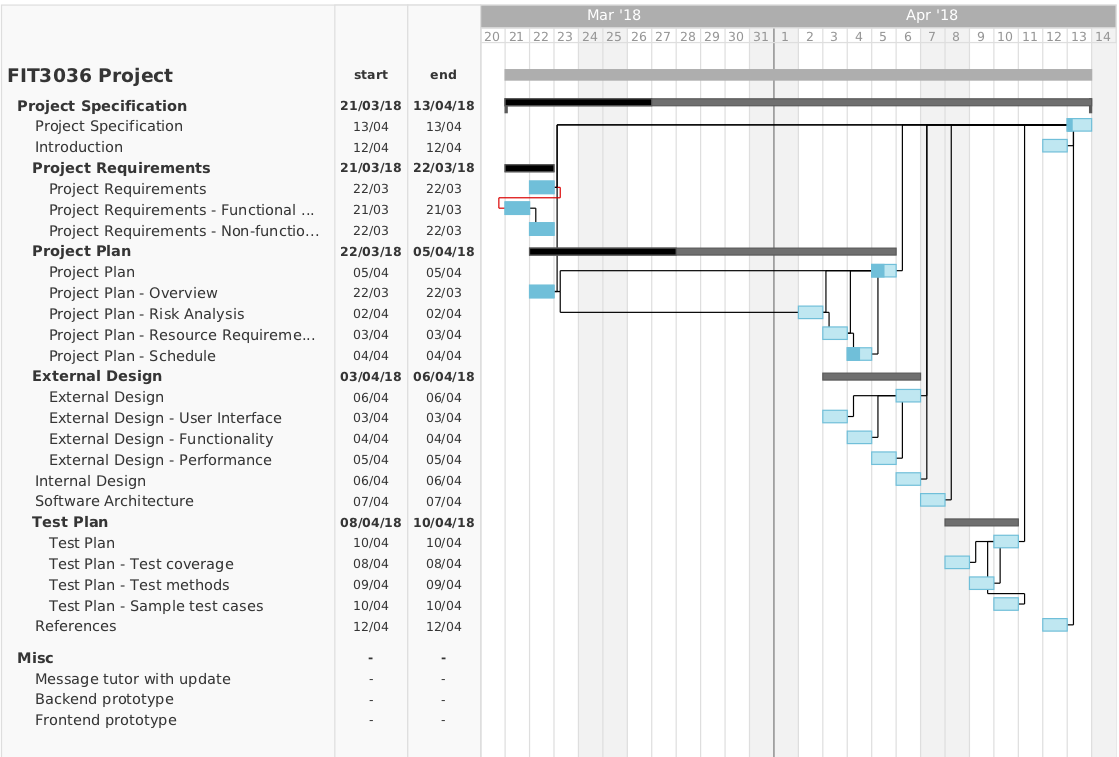
\includegraphics[width=\textwidth]{gantt-chart}
  \caption{Gantt chart}\label{fig:gantt}
\end{figure}

\section{External Design}

The external design includes the user interface, functionality and performance.

\subsection{User Interface}

Created mock-up as seen in figure~\ref{fig:mockup}, main features are:

\begin{itemize}
  \item Open webpage and user is presented with a large render of Google Maps.
    There is a square that can be positioned and sized over the map for the user
    to select the area to calculate.
  \item A calculation shows the total area of the shape over the map. This is
    updated whenever the user resizes or moves the square.
  \item The user then pushes the ``Calculate'' button to generate the surface
    area of the roads within the square.
  \item There is help information on the page.
\end{itemize}

\begin{figure}[H]
  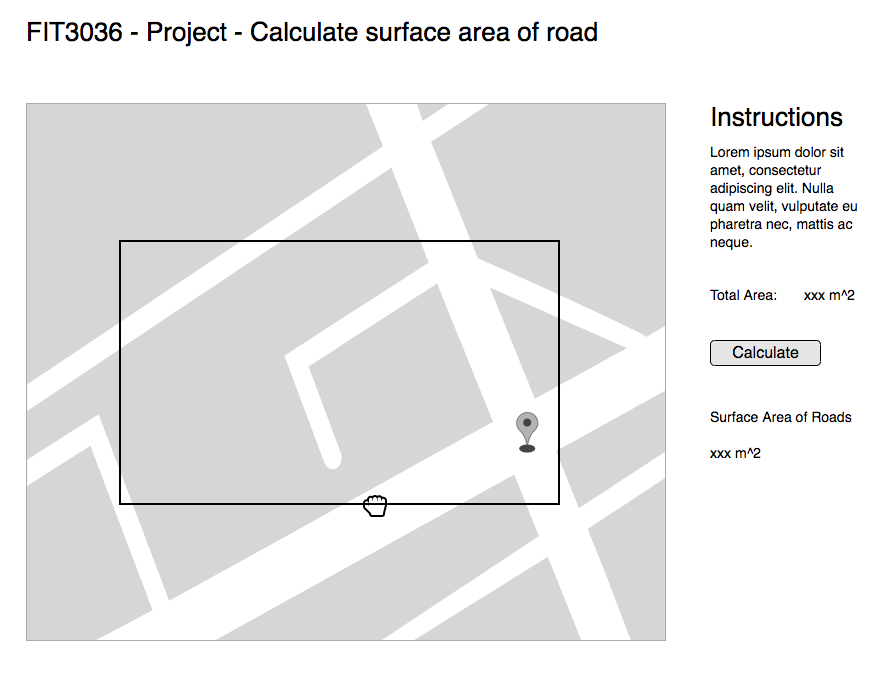
\includegraphics[width=\textwidth]{UI-mockup}
  \caption{Application Mock-up}\label{fig:mockup}
\end{figure}

\subsection{Functionality}

An API will be created that will take 4 position parameters, each boundary is
made up of a Latitude and Longitude. This data is used to call the  Open Street
Maps API \autocite{osm:14} to return data about all of the streets within the
area.

This is then passed to a method that will use the Haversine distance calculation
\autocite{hav:8} to calculate distance between all of the nodes. If number of
lanes information is provided then this is multiplied by by the default lane
width within Australia (3.5m) \autocite{lane:9} if not then we are assuming that
the road is only 2 lanes wide. This is then summed and returned.

Another API is exposed for the front-end UI, it calculates the total area of the
of the shape over the map. This has been included to help improve the UI.\@ The
API method will take 4 position arguments, each a boundary, made up of a single
latitude and longitude. This will calculate the surface area of the 4 points and
return the area \autocite{math:10}.

\subsection{Performance}

When considering performance the two main points are time and space.

\paragraph{Time:}

We would like the response from the API to calculate the area of the square to
be very fast $(< 0.5s)$ as this will run whenever, the area is changed.

The main method that will calculate the total surface area of the all of the
roads will also need to be sum what fast as we don't want the user to have to
wait a long time while this is calculated $(< 30s)$.

\paragraph{Space:}

The back-end code which runs on AWS Lambda, can run between 128--3008MB memory
to run the method. The default is 1024MB which is what we will be using.

\section{Internal Design}

The two main functions of the system are to calculate the total surface area of
the selected area and to calculate the surface area of the roads within the same
area.

\paragraph{Calculate Total Surface Area:}

These steps below are outlined in figure~\ref{fig:seq-total-area}

\begin{enumerate}
  \item User drags or resizes square in Map.
  \item These parameters are sent to the back-end service.
  \item This calculates the total surface area.
  \item This is returned to the user.
\end{enumerate}

\begin{figure}[H]
  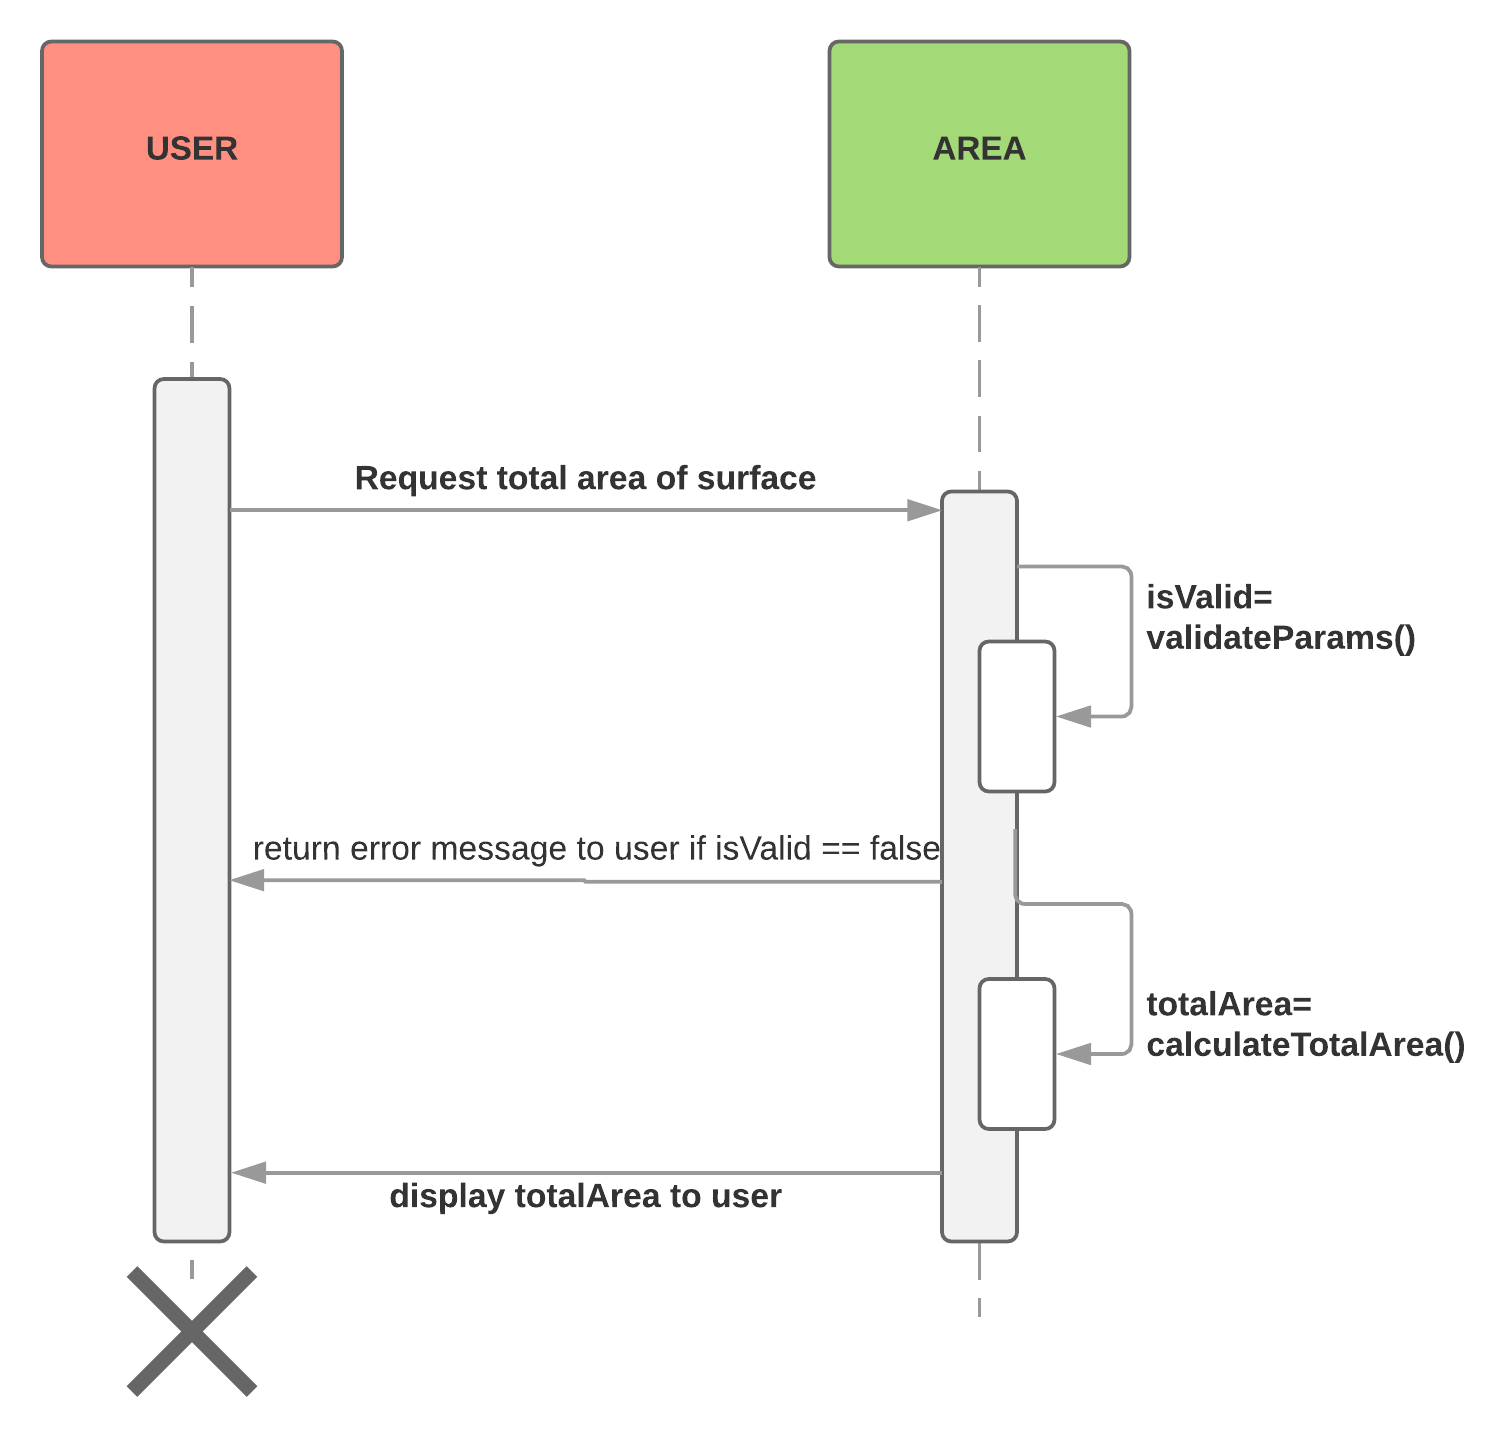
\includegraphics[width=\textwidth]{sequence-diagram-calculate-total-surface-area}
  \caption{Sequence Diagram --- Calculate Total Surface
  Area}\label{fig:seq-total-area}
\end{figure}

\paragraph{Calculate Total Surface Area of Roads:}

These steps below are outlined in figure~\ref{fig:seq-total-area-roads}

\begin{enumerate}
  \item User requests to calculate total surface area of roads.
  \item These parameters are sent to the back-end service.
  \item These are used to call OpenStreetMap API
  \item It then iterates over data and calculates the distance of all of the
    roads.
  \item The area of these roads is then calculated with lane width.
  \item These results are summed.
  \item This is returned to the user.
\end{enumerate}

\begin{figure}[H]
  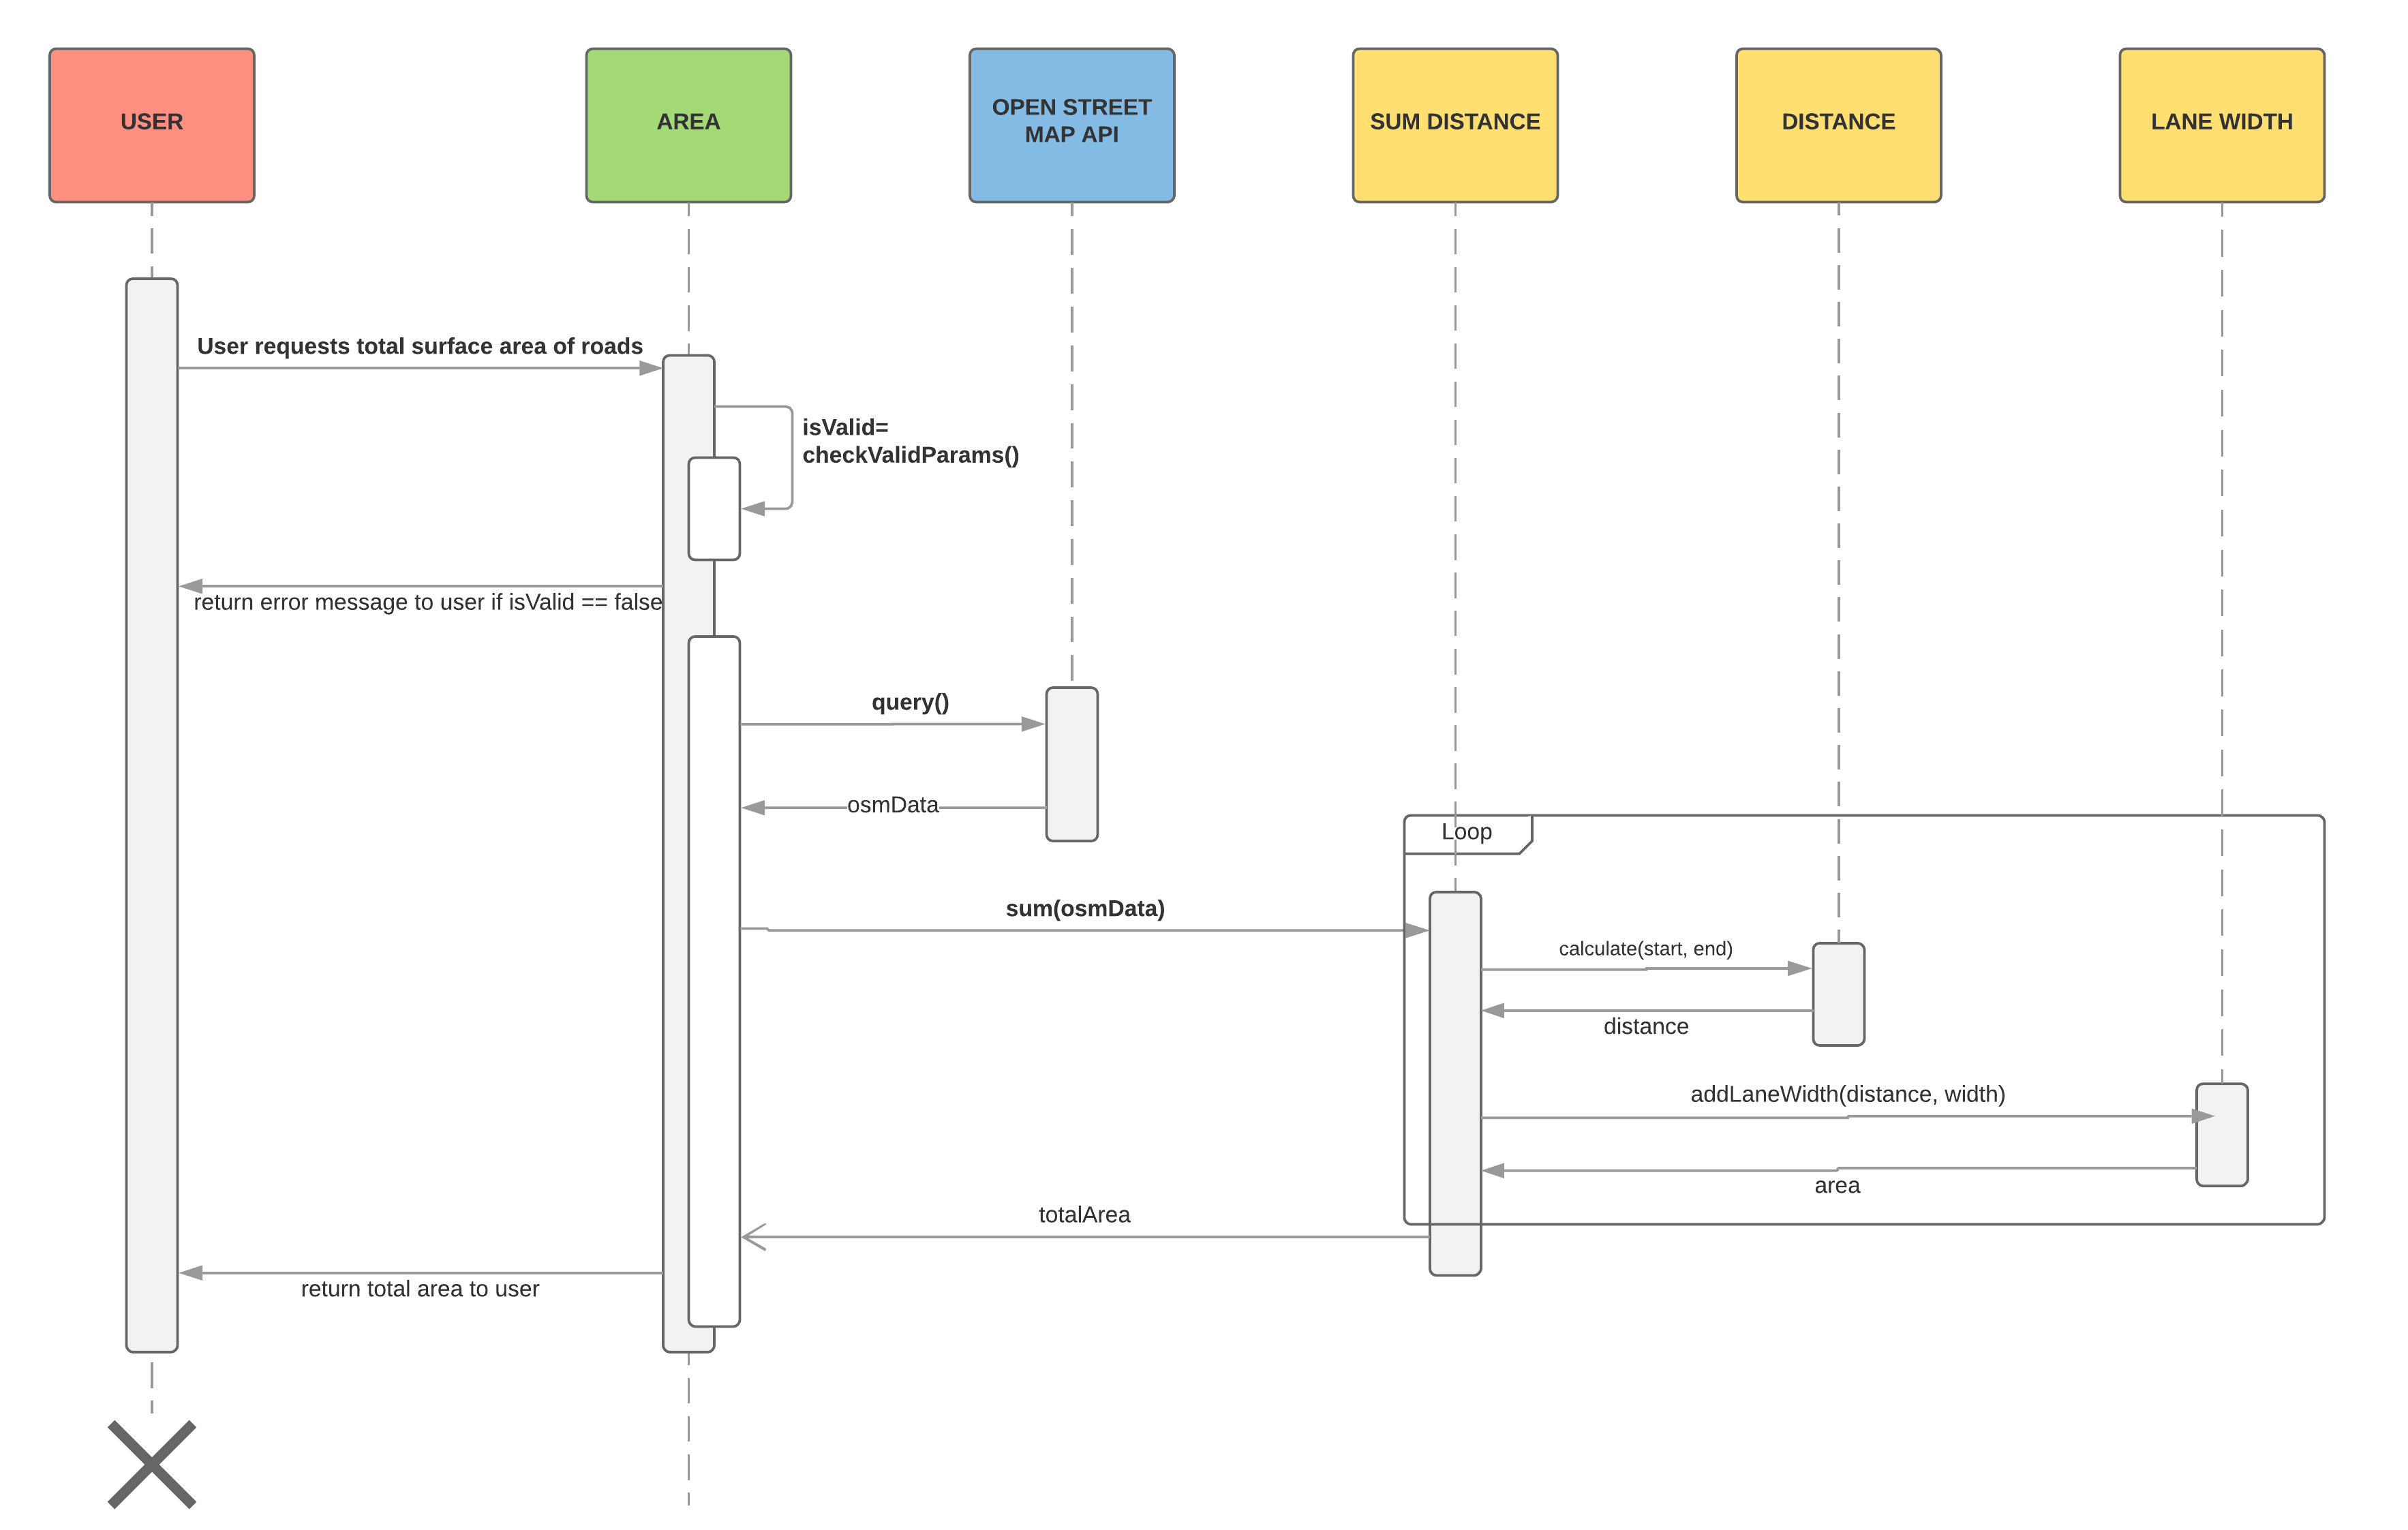
\includegraphics[width=\textwidth]{sequence-diagram-calculate-total-surface-area-of-roads}
  \caption{Sequence Diagram --- Calculate Total Surface Area of
  Roads}\label{fig:seq-total-area-roads}
\end{figure}

\section{Software Architecture}

Figure~\ref{fig-class-diagram} shows how architecture of the back-end code. It
is broken up into 4 main classes, which calculate area, sum data, calculate
distance and calculate the area of a road.

\begin{figure}[H]
  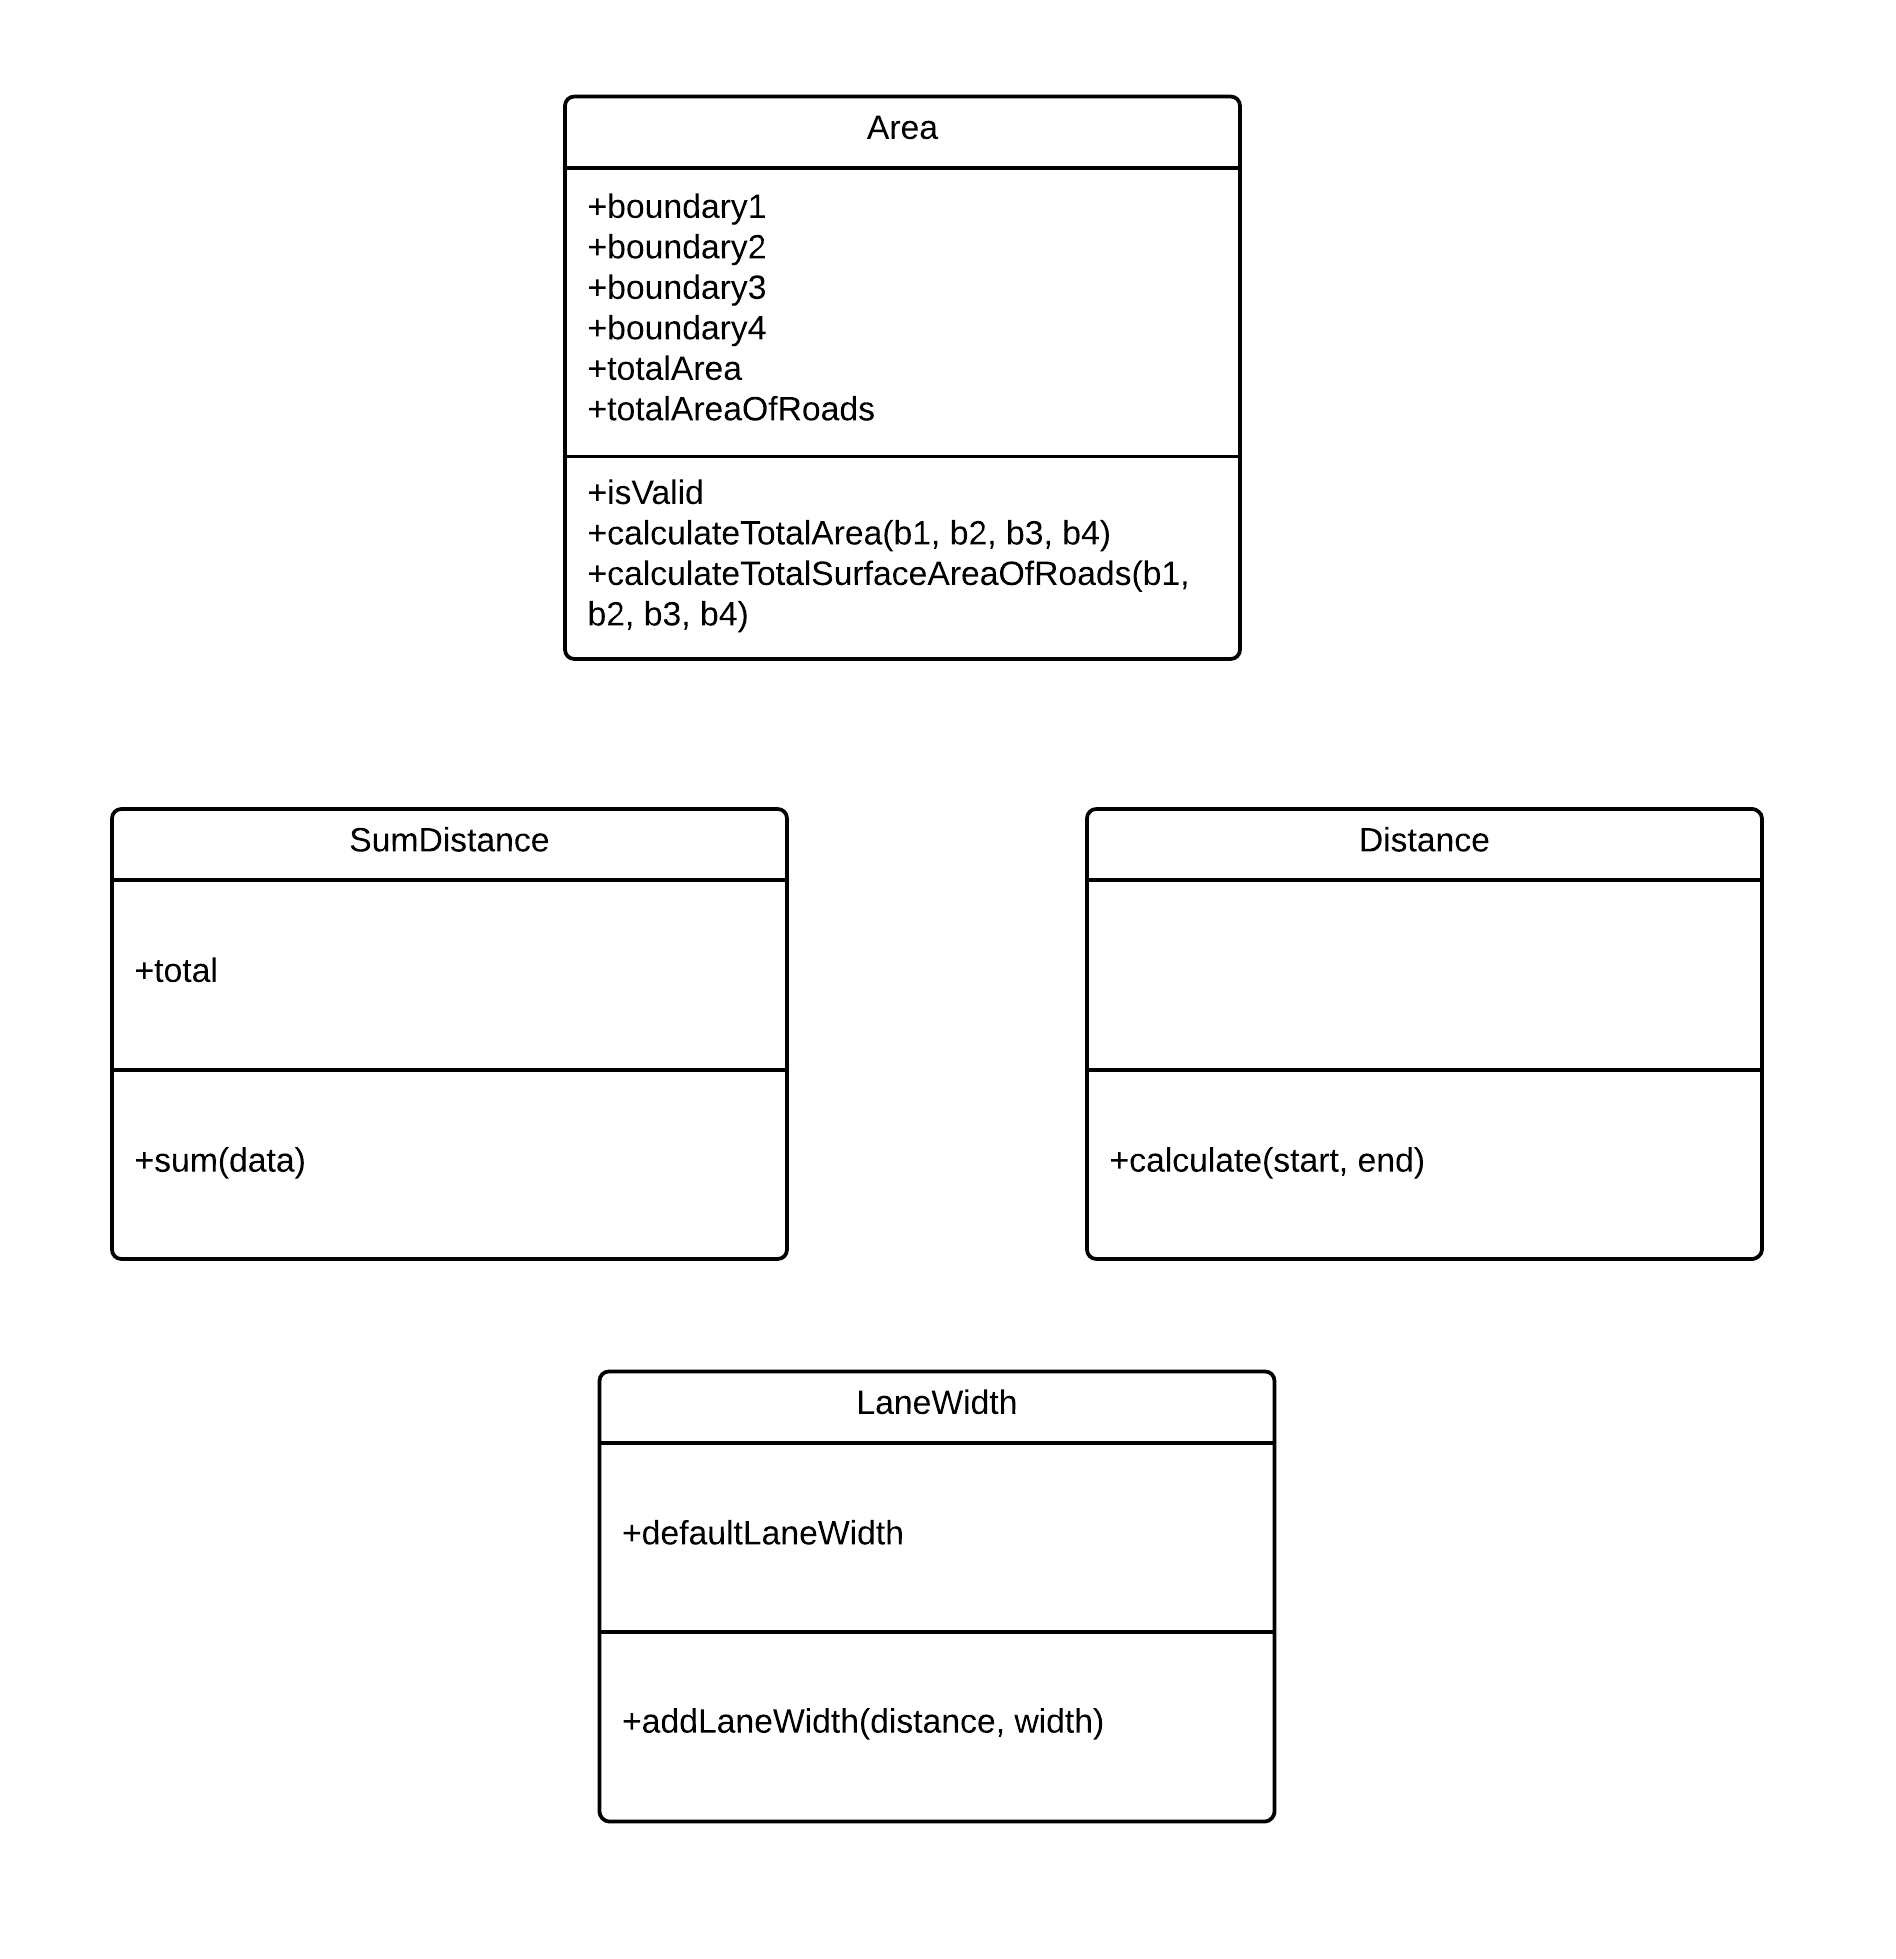
\includegraphics[width=\textwidth]{class-diagram}
  \caption{Class Diagram}\label{fig:class-diagram}
\end{figure}

\section{Test Plan}

Test plan for this project includes test coverage, test methods and the sample
test cases that will be used.

\subsection{Test coverage}

We are going to use Jest \autocite{jest:11} and react-testing-library
\autocite{rtl:12} to test the front-end components.

To test the back-end code we can use the inbuilt testing package in Go
\autocite{go:13}.

These will automatically be run through development using test runners to run on
code change.

Tests will also be run automatically through the CI/CD service before deployment
to ensure that that code is only deployed if the tests have passed.

\subsection{Test methods}

To ensure that the project is fully tested it will use a variety of tests.

\begin{itemize}
  \item Unit tests on all class methods. This verifies that the individual
    functions behave as expected.
  \item Integration tests for API back-end to ensure that correct response is
    returned for known parameters.
  \item Unit test front-end components to ensure that they behave and interact
    in the correct manor.
  \item Acceptance tests to make sure all requirements are met.
  \item Able to generate test coverage reports for front end and back end code.
    $80-100\%$ test coverage is acceptable.
  \item System tests will test the system as a whole and test the entire
    functionality.
\end{itemize}

\subsection{Sample test cases}

We are going to create test plans that will cover the main functionality of the
program. These will include:

\begin{itemize}
  \item Test a known Area to calculate the total area.
  \item Test a known Distance to know the length of it.
  \item Test a known Area to sanity check the surface area of the roads within
    it.
\end{itemize}

\pagebreak

\section{References}

\printbibliography{}

\end{document}
